\chapter{Сдавливание круглого идеально жесткопластического слоя}\label{ch:ch1}
%При пластической деформации тонких слоев в процессах прессования актуальна проблема получения изделий заданной точности. Существенное влияние на конечную геометрию детали оказывает деформируемость сдавливающих поверхностей. Из-за больших нагрузок на инструмент, деформация последнего может быть соизмерима с толщиной обрабатываемого слоя. Этим обуславливается важность знания распределения силовых факторов в зоне контакта. Для случая сжатия плоской полосы модельной задачей является классическая задача Прандтля \autocite{Prandtl:1948}. Её осесимметричным аналогом является задача о сдавливании идеально жесткопластического круглого слоя \autocite{Georgievsky:2008}. Для данной задачи исследуется влияние динамических эффектов в процессе прессования. Материалы главы содержатся в публикации \autocite{Shabaykin:2017}.
При пластической деформации тонких заготовок в процессах прессования возникает потребность получения изделий заданной точности. Существенное влияние на конечную геометрию детали оказывает деформируемость сдавливающих поверхностей. Вследствие значительных нагрузок на инструмент деформация последнего может оказаться соизмерима с толщиной обрабатываемого слоя. Этим обуславливается важность получения полей распределения силовых факторов в зоне контакта. Для случая сжатия плоской полосы, модельной задачей является классическая задача Прандтля \autocite{Prandtl:1948}. Её осесимметричным аналогом является задача о сдавливании идеально жесткопластического круглого слоя \autocite{Georgievsky:2008}. В данной постановке задачи исследуется влияние динамических эффектов в процессе формирования изделия методом прессования. Материалы главы содержатся в публикации \autocite{Shabaykin:2017}.
%Обеспечение заданной точности изделий, получаемых методом прессовки (прессования) актуализируют задачу определения пластической деформации тонких слоёв материала.

\section{Постановка задачи и асимптотические разложения}\label{sec:ch1/sec1}

Пренебрегая начальными упругими деформациями, вязкостью и незначительным упрочнением, материал, имеющий плотность $\varrho$, полагается несжимаемым идеально жесткопластическим, удовлетворяющим тензорно линейным определяющим соотношениям и скалярному определяющему соотношению -- квадратичному критерию Мизеса-Генки $\sigma_{u} = \sigma_{s}$, где $\sigma_{u} = \sqrt{\utilde{s} : \utilde{s}}$ -- интенсивность напряжения, $\utilde{s}$ -- девиатор напряжения, $\sigma_{s}$ -- предел текучести.

Пусть течение происходит в области
\begin{equation}
  \Omega_{t} = \{0 \le r \le R(t), -h(t) \le z \le h(t), 0 \le \theta < 2\pi\},
\end{equation}
с границей $\partial\Omega = \Gamma = \Gamma_{1} \cup \Gamma_{2} \cup \Gamma_{3}$, причем $h(t) \ll R(t)$ для любого $t \ge 0$. В начальный момент времени область, занятая материалом, имела вид
\begin{equation}
  \Omega_{0} = \{0 \le r \le R_{0}, -h_{0} \le z \le h_{0}, 0 \le \theta < 2\pi\}, \quad \partial\Omega_{0} = \Gamma_{0}
\end{equation}
поэтому в силу несжимаемости $R^{2} h=R^{2}_{0} h_{0}$.

\begin{figure}[ht]
  \centerfloat{
    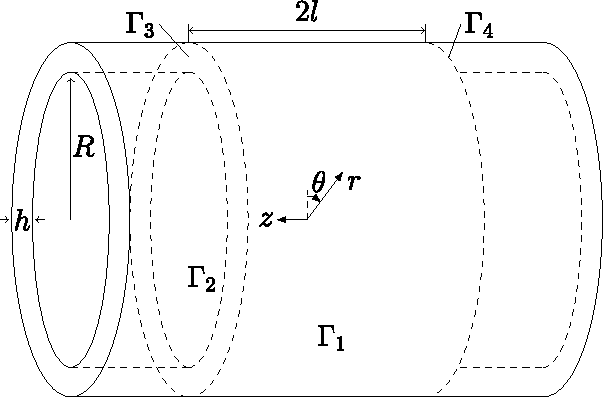
\includegraphics[width=0.6\linewidth]{./ch1/layer}
  }
  \caption{Представление круглого слоя}
  \label{fig:ch1/layer}
\end{figure}
Взаимную скорость сближения плит обозначим $2V$, поэтому кинематическое условие непротекания сквозь границы $\Gamma_{1}$ и $\Gamma_{2}$ имеет вид
\begin{equation}
  \label{eq:ch1/sec1/boundary/kinematic}
  v_{z}\lvert_{z=\pm h} = \mp V
\end{equation}
Касательная составляющая скорости (в данном случае $v_{r}$) на указанных границах идеальной среды, как известно, не задаётся.

В некоторый момент времени $0 < t < h_{0}/V = t_*$, где $t_*$ -- момент схлопывания слоя, относительно шести функций -- независимых компонент девиатора напряжений $s_{rr}$, $s_{rz}$ и $s_{\theta\theta}$, давления $p$ и компонент скорости $v_{r}$ и $v_{z}$ -- должна выполнятся замкнутая система уравнений динамической теории идеальной пластичности для цилиндрических координат:
\begin{gather}
  \label{eqs:ch1/sec1/general/motion:1}
  -p_{,r}+s_{rr,r}+s_{rz,z}+\frac{s_{rr}-s_{\theta\theta}}{r} = \varrho \left(v_{r;t}+v_{r} v_{r,r} + v_{z} v_{r,z} \right)
  \\
  \label{eqs:ch1/sec1/general/motion:2}
  -p_{,z}+s_{rz,r}+\frac{s_{rz}}{r}-(s_{rr}+s_{\theta\theta})_{,z} = \varrho \left(v_{z;t}+v_{r} v_{z,r} + v_{z} v_{z,z} \right)
  \\
  \label{eqs:ch1/sec1/general/plasticity}
  s^2_{rr}+s^2_{\theta\theta}+s_{rr} s_{\theta\theta} + s^2_{rz}=\tau^2_{s}
  \\
  \label{eqs:ch1/sec1/general/coax:1}
  s_{rr} \frac{v_{r}}{r} = s_{\theta\theta} v_{r,r}
  \\
  \label{eqs:ch1/sec1/general/coax:2}
  s_{rr} (v_{r,z}+v_{z,r}) = 2 s_{rz} v_{r,r}
  \\
  \label{eqs:ch1/sec1/general/uncompress}
  v_{r,r}+\frac{v_{r}}{r}+v_{z,z} = 0
\end{gather}

\expandafter\gdef\csname eqs:ch1/sec1/general\endcsname{eqs:ch1/sec1/general/motion:1,eqs:ch1/sec1/general/motion:2,eqs:ch1/sec1/general/plasticity,eqs:ch1/sec1/general/coax:1,eqs:ch1/sec1/general/coax:2,eqs:ch1/sec1/general/uncompress}
Кроме выполнения условия \cref{eq:ch1/sec1/boundary/kinematic} на жестких контактирующих поверхностях потребуем, что бы модуль касательного напряжения $s_{rz}$ достигал на границах $\Gamma_{1}$ и $\Gamma_{2}$ своего максимального значения:
\begin{equation}
  \label{eq:ch1/sec1/boundary/force}
  \lvert s_{rz}\lvert_{z=\pm h} = m(r) \tau_{s}, \quad 0 < m \le 1,
\end{equation}
где $m$ -- функция, удовлетворяющая уравнению первого порядка с разделяющимися переменными \autocite{Georgievsky:2008}:
\begin{equation}
  \label{eq:ch1/sec1/m}
  \frac{dm}{dr}=\frac{m}{2r}\left(1+\frac{m\sqrt{1-m^2}}{\arcsin m}\right)
\end{equation}
Из \cref{eq:ch1/sec1/m} видно, что функция $m$ не может быть тождественно равна отличной от нуля константе. Это существенно усложняет и отличает настоящее решение от соответствующего решения классической задачи Прандтля, в постановке которой $m = \pm m_0$, где параметр $m_0$  имеет смысл коэффициента шероховатости плит.

В реальном процессе сжатия слоя граница $\Gamma_{3}$, естественно, свободна от напряжений, однако в математической постановке рассматриваемой здесь краевой задачи в её классическом варианте данное условие не ставится. Поэтому других, помимо \cref{eq:ch1/sec1/boundary/kinematic, eq:ch1/sec1/boundary/force}, граничных условий в задаче не предполагается, а область вблизи границы $\Gamma_{3}$ (на расстояниях порядка $h$) трактуется как зона краевого эффекта.

Введем малый параметр $\alpha = \frac{h(t)}{R(t)} \ll 1$ и проведем разложение всех неизвестных величин, входящих в систему уравнений \cref{\csname eqs:ch1/sec1/general\endcsname}, в ряды по целым степеням параметра:
\begin{gather}
  \label{eqs:ch1/series/vr}
  v_{r}\left(r, z, t\right) = V \sum_{k=-N}^{\infty}{\alpha^{k} \; \uindex{v}{k}_{r}}, \quad N \ge 1
  \\
  \label{eqs:ch1/series/vz}
  v_{z}\left(r, z, t\right) = V \sum_{k=0}^{\infty}{\alpha^{k} \; \uindex{v}{k}_{z}}
  \\
  \label{eqs:ch1/series/sij}
  s_{ij}\left(r, z, t\right) = \tau_{s} \sum_{k=0}^{\infty}{\alpha^{k} \; \uindex{s}{k}_{ij}}, \quad (ij)\in\{rr, rz, \theta\theta\}
  \\
  \label{eqs:ch1/series/p}
  p\left(r, z, t \right) = \tau_{s} \sum_{k=-M}^{\infty}{\alpha^{k} \; \uindex{p}{k}}, \quad M \ge 1
\end{gather}

\expandafter\gdef\csname eqs:ch1/series\endcsname{eqs:ch1/series/vr,eqs:ch1/series/vz,eqs:ch1/series/sij,eqs:ch1/series/p}
Коэффициенты рядов \cref{\csname eqs:ch1/series\endcsname} -- безразмерны и являются функциями безразмерных координат $\rho, \xi, \tau$
\begin{equation}
  \label{eq:ch1/coordinates}
  \rho = \frac{r}{R} = \frac{\alpha r}{h}, \quad \xi = \frac{z}{h}, \quad \tau = V \frac{t}{h}
\end{equation}
Наличие в \cref{\csname eqs:ch1/series\endcsname} членов $\alpha^{-n} \; \uindex{v}{-n}_{r}$ и $\alpha^{-m} \; \uindex{p}{-m}$ обусловлено стремлением $v_{r}$ и $p$ к бесконечности, при $\alpha\rightarrow 0$, что ясно из физических соображений.
Обратимся к геометрическому условию несжимаемости и выразим малый параметр и координаты \cref{eq:ch1/coordinates} как эволюционные функции:

\begin{gather}
  \left(R^2 h\right)^. = 0, \quad \dot{R} = -\dot{h} \frac{R}{2h}= V \frac{R}{2h}\nonumber
  \\
  \dot{\alpha} = \left(\frac{h}{R}\right)^. = \frac{\dot{h}R - h\dot{R}}{h^2} = -\frac{3 V}{2 h} \alpha
  \\
  \dot{\rho} = \left(\frac{\alpha r}{h}\right)^. = r \frac{\dot{\alpha} h - \alpha \dot{h}}{h^2} = -\frac{V}{2h}\rho
  \\
  \dot{\xi} = \left(\frac{z}{h}\right)^. = -\frac{z \dot{h}}{h^2} = \frac{V}{h}\xi
  \\
  \dot{\tau} = \left(V \frac{t}{h}\right)^. = V \frac{h - t\dot{h}}{h^2} = \frac{V}{h} \left(1+\tau\right)
\end{gather}

Подставляя выражения \cref{\csname eqs:ch1/series\endcsname} в систему \cref{\csname eqs:ch1/sec1/general\endcsname} и учитывая, что полная производная по времени представляется в виде
\begin{equation*}
  \uindex{v}{k}_{i;t} = \uindex{v}{k}_{i,\rho} \dot{\rho} + \uindex{v}{k}_{i,\xi} \dot{\xi} + \uindex{v}{k}_{i,\tau} \dot{\tau}
\end{equation*}
получим следующую систему:
\begingroup
\allowdisplaybreaks
\begin{gather}
  \label{eqs:ch1/sec1/substituted/motion:1}
  \begin{multlined}
    -\sum_{k=-M}^{\infty}{\alpha^{k+1} \; \uindex{p}{k}_{,\rho}} +
    \sum_{k=0}^{\infty}{\alpha^{k}\left(
    \alpha \ \uindex{s}{k}_{rr,\rho} +
    \uindex{s}{k}_{rz,\xi} +
    \frac{\alpha}{\rho}\left(\ \uindex{s}{k}_{rr} - \uindex{s}{k}_{\theta\theta}\right)
    \right)} \unl{=}
    \frac{\varrho V^2}{\tau_{s}}\left(
    \sum_{k=-N}^{\infty}{\alpha^{k}\left(
      -\uindex{v}{k}_{r,\rho} \frac{\rho}{2} +
      \uindex{v}{k}_{r,\xi} \xi +
      \uindex{v}{k}_{r,\tau} \left(1+\tau\right) -
      \frac{3 k}{2} \ \uindex{v}{k}_{r}
      \right)}
    \unl[1]{+}
    \sum_{k=-N}^{\infty}{\alpha^{k} \; \uindex{v}{k}_{r}} \sum_{k=-N}^{\infty}{\alpha^{k+1} \; \uindex{v}{k}_{r,\rho}} +
    \sum_{k=0}^{\infty}{\alpha^{k} \; \uindex{v}{k}_{z}} \sum_{k=-N}^{\infty}{\alpha^{k} \; \uindex{v}{k}_{r,\xi}}
    \right)
  \end{multlined}
  \\
  \label{eqs:ch1/sec1/substituted/motion:2}
  \begin{multlined}
    -\sum_{k=-M}^{\infty}{\alpha^{k} \; \uindex{p}{k}_{,\xi}} + \sum_{k=0}^{\infty}{\alpha^{k}\left(
    \alpha \ \uindex{s}{k}_{rz,\rho} +
    \frac{\alpha}{\rho} \ \uindex{s}{k}_{rz} -
    \left(\ \uindex{s}{k}_{rr,\xi} + \uindex{s}{k}_{\theta\theta,\xi}\right)
    \right)} \unl{=} \frac{\varrho V^2}{\tau_{s}}\left(
    \sum_{k=0}^{\infty}{\alpha^{k}\left(
      -\uindex{v}{k}_{z,\rho} \frac{\rho}{2} +
      \uindex{v}{k}_{z,\xi} \xi +
      \uindex{v}{k}_{z,\tau} \left(1+\tau\right) -
      \frac{3 k}{2} \ \uindex{v}{k}_{z}
      \right)} \unl[1]{+}  \sum_{k=-N}^{\infty}{\alpha^{k} \; \uindex{v}{k}_{r}} \sum_{k=0}^{\infty}{\alpha^{k+1} \; \uindex{v}{k}_{z,\rho}} +
    \sum_{k=0}^{\infty}{\alpha^{k} \; \uindex{v}{k}_{z}} \sum_{k=0}^{\infty}{\alpha^{k} \; \uindex{v}{k}_{z,\xi}}
    \right)
  \end{multlined}
  \\
  \label{eqs:ch1/sec1/substituted/plasticity}
  \begin{multlined}
    \left(\sum_{k=0}^{\infty}{\alpha^{k} \; \uindex{s}{k}_{rr}}\right)^2+
    \left(\sum_{k=0}^{\infty}{\alpha^{k} \; \uindex{s}{k}_{\theta\theta}}\right) \unl{+}
    \sum_{k=0}^{\infty}{\alpha^{k} \; \uindex{s}{k}_{rr}} \sum_{k=0}^{\infty}{\alpha^{k} \; \uindex{s}{k}_{\theta\theta}}+
    \left(\sum_{k=0}^{\infty}{\alpha^{k} \; \uindex{s}{k}_{rz}}\right)^2 = 1
  \end{multlined}
  \\
  \label{eqs:ch1/sec1/substituted/coax:1}
  \sum_{k=0}^{\infty}{\alpha^{k} \; \uindex{s}{k}_{rr}} \frac{\alpha}{\rho} \sum_{k=-N}^{\infty}{\alpha^{k} \; \uindex{v}{k}_{r}} =
  \sum_{k=0}^{\infty}{\alpha^{k} \; \uindex{s}{k}_{\theta\theta}} \sum_{k=-N}^{\infty}{\alpha^{k+1} \; \uindex{v}{k}_{r,\rho}}
  \\
  \label{eqs:ch1/sec1/substituted/coax:2}
  \sum_{k=0}^{\infty}{\alpha^{k} \; \uindex{s}{k}_{rr}} \left(
  \sum_{k=-N}^{\infty}{\alpha^{k} \; \uindex{v}{k}_{r,\xi}} +
  \sum_{k=0}^{\infty}{\alpha^{k+1} \; \uindex{v}{k}_{z,\rho}}
  \right) =
  2 \sum_{k=0}^{\infty}{\alpha^{k} \; \uindex{s}{k}_{rz}} \sum_{k=-N}^{\infty}{\alpha^{k+1} \; \uindex{v}{k}_{r,\rho}}
  \\
  \label{eqs:ch1/sec1/substituted/uncompress}
  \sum_{k=-N}^{\infty}{\alpha^{k+1} \; \uindex{v}{k}_{r,\rho}}+
  \frac{\alpha}{\rho}\sum_{k=-N}^{\infty}{\alpha^{k} \; \uindex{v}{k}_{r}}+
  \sum_{k=0}^{\infty}{\alpha^{k} \; \uindex{v}{k}_{z,\xi}} = 0
\end{gather}

\expandafter\gdef\csname eqs:ch1/sec1/substituted\endcsname{eqs:ch1/sec1/substituted/motion:1,eqs:ch1/sec1/substituted/motion:2,eqs:ch1/sec1/substituted/plasticity,eqs:ch1/sec1/substituted/coax:1,eqs:ch1/sec1/substituted/coax:2,eqs:ch1/sec1/substituted/uncompress}
Возникший в правой части уравнений \cref{eqs:ch1/sec1/substituted/motion:1, eqs:ch1/sec1/substituted/motion:2} коэффициент равен обратному числу Эйлера
\begin{equation*}
  \text{Eu}^{-1} = \frac{\varrho V^2}{\tau_{s}}.
\end{equation*}
Данная величина мала \todo{почему?}и как видно из её определения фиксирована. По сравнению с ней порядок малости $\alpha(t)$ при течении времени от 0 до $t_*$ растёт до бесконечности. Это позволяет записать
\begin{equation*}
  \text{Eu}^{-1} = O\left(\alpha^\beta(t)\right), \text{ причем } \beta \rightarrow 0 \text{ при } t \rightarrow t_*
\end{equation*}
\endgroup
Применительно к динамическому анализу интерес представляет $0 < \beta \le 2$. Отыскание решений проведем для целочисленных значений входящих в этот диапазон.

Обратимся к системе двух последних уравнений \cref{eqs:ch1/sec1/substituted/coax:2, eqs:ch1/sec1/substituted/uncompress}. Из \cref{eqs:ch1/sec1/substituted/coax:2} сразу следует, что $\uindex{v}{-N}_{r,\xi} = 0$, а решая дифференциальное уравнение \cref{eqs:ch1/sec1/substituted/uncompress} и требуя конечности членов разложения, получаем, что $\uindex{v}{-N}_{r} = 0$. Аналогичные рассуждения применимы последовательно для $\uindex{v}{-N+1}_{r}$, затем $\uindex{v}{-N+2}_{r}$ и далее вплоть до $\uindex{v}{-2}_{r}$.
Учитывая, что первый ненулевой член радиальной компоненты скорости $\uindex{v}{-1}_{r}$, и принимая, что $\beta \ge 1$ определим из уравнений \cref{eqs:ch1/sec1/substituted/motion:1, eqs:ch1/sec1/substituted/motion:2} порядок малости для функции давления $p$. Для $M \ge 2$ имеем:
\begin{equation*}
  -\uindex{p}{-M}_{,\rho} = 0, \quad -\uindex{p}{-M}_{,\xi} = 0 \text{ и, следовательно, } \ \uindex{p}{-M} = \uindex{p}{-M}_{0}(\tau)
\end{equation*}
Здесь $\uindex{p}{-M}_{0}$ -- гидростатическая постоянная, не дающая вклад в уравнение движения и однозначно определяемая заданием внешнего давления. Поэтому, без ограничения общности, можно считать, что $M=1$.

Аналогично \cref{eq:ch1/sec1/m} введем коэффициент шероховатости поверхности, зависящий от безразмерного радиуса:
\begin{equation}
  \label{eq:ch1/sec1/mu}
  \mu(\rho) = m(r/R), \quad \frac{d\mu}{d\rho}=\frac{\mu}{2\rho}\left(1+\frac{\mu\sqrt{1-\mu^2}}{\arcsin\mu}\right)
\end{equation}
Вообще говоря, уравнение \cref{eq:ch1/sec1/mu} определяет функцию $\mu(\rho)$ с точностью до умножения на константу. Её график, при условии $\mu(1) = 1$, приведен на рисунке ниже:
\begin{figure}[ht]
  \centerfloat{
    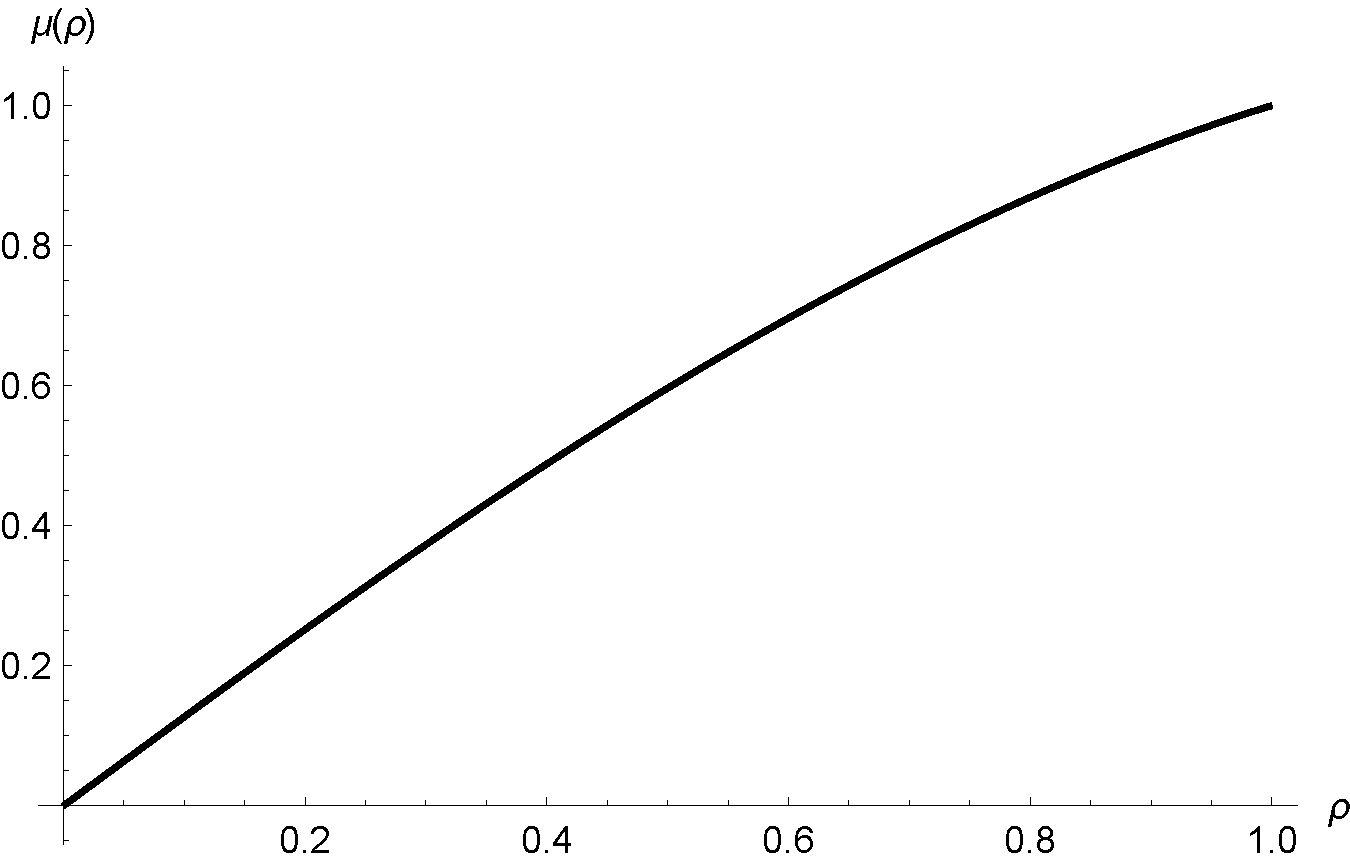
\includegraphics[scale=1.3]{./ch1/mu}
  }
  \caption{Вид функции $\mu(\rho)$, при $\mu(1)=1$}
  \label{fig:ch1/mu}
\end{figure}

Вид функции $\mu(\rho)$ при другом граничном условии на правом конце может быть получен масштабированием по оси $\rho$.

\section{Построение решения}\label{sec:ch1/sec2}
\subsection{Переход от квазистатического к динамическому режиму деформирования}\label{subsec:ch1/sec2/sub1}

Рассмотрим случай $\beta=2$, который соответствует моменту перехода от квазистатического к динамическому режиму деформирования.

Положим $\text{Eu}^{-1} = C_2 \alpha^2$ и последовательно приравняем коэффициенты правых и левых частей уравнений системы \cref{\csname eqs:ch1/sec1/substituted\endcsname} при $a^{-1}$ и $\alpha^0$:
\begingroup
\allowdisplaybreaks
\begin{gather}
  \label{eqs:ch1/sec2/sub1/-1/motion:2}
  -\uindex{p}{-1}_{,\xi} = 0
  \\
  \label{eqs:ch1/sec2/sub1/-1/coax:2}
  \uindex{s}{0}_{rr} \; \uindex{v}{-1}_{r,\xi} = 0
  \\
  \label{eqs:ch1/sec2/sub1/0/motion:1}
  -\uindex{p}{-1}_{,\rho}+\uindex{s}{0}_{rz,\xi} = 0
  \\
  \label{eqs:ch1/sec2/sub1/0/motion:2}
  -\uindex{p}{0}_{,\xi} - \uindex{s}{0}_{rr,\xi} - \uindex{s}{0}_{\theta\theta,\xi} = 0
  \\
  \label{eqs:ch1/sec2/sub1/0/plasticity}
  \left(\uindex{s}{0}_{rr}\right)^2 + \left(\uindex{s}{0}_{\theta\theta}\right)^2 + \uindex{s}{0}_{rr}\; \uindex{s}{0}_{\theta\theta} + \left(\uindex{s}{0}_{rz}\right)^2 = 1
  \\
  \label{eqs:ch1/sec2/sub1/0/coax:1}
  \uindex{s}{0}_{rr} \; \uindex{v}{-1}_{r} / \rho = \uindex{s}{0}_{\theta\theta} \uindex{v}{-1}_{r,\rho}
  \\
  \label{eqs:ch1/sec2/sub1/0/coax:2}
  \uindex{s}{0}_{rr} \; \uindex{v}{0}_{r,\xi} = 2 \uindex{s}{0}_{rz} \; \uindex{v}{-1}_{r,\rho}
  \\
  \label{eqs:ch1/sec2/sub1/0/uncompress}
  \uindex{v}{-1}_{r,\rho} + \uindex{v}{-1}_{r} / \rho + \uindex{v}{0}_{z,\xi} = 0
\end{gather}
\endgroup
Граничные условия \cref{eq:ch1/sec1/boundary/kinematic, eq:ch1/sec1/boundary/force} при этом примут вид
\begin{equation}
  \label{eq:ch1/sec1/sub1/boundary/0}
  \uindex{v}{0}_{z}\lvert_{\xi=\pm 1} = \mp 1, \quad \lvert \uindex{s}{0}_{rz}\lvert_{\xi=\pm 1} = \mu(\rho)
\end{equation}
Из уравнений \cref{eqs:ch1/sec2/sub1/-1/motion:2, eqs:ch1/sec2/sub1/-1/coax:2} вытекает
\begin{equation*}
  \uindex{p}{-1} = \uindex{f}{-1}_{p}(\rho, \tau), \quad \uindex{v}{-1}_{r} = \uindex{f}{-1}_{v_{r}}(\rho, \tau).
\end{equation*}
Подставив выражение $\uindex{v}{-1}_{r}$ в уравнение \cref{eqs:ch1/sec2/sub1/0/uncompress} и решив дифференциальное уравнение, получим выражение для $\uindex{v}{0}_{z}$:
\begin{equation*}
  \uindex{v}{0}_{z} = \uindex{f}{0}_{v_{z}}(\rho, \tau) -\xi \left(\ \uindex{f}{-1}_{v_{r},\rho} + \uindex{f}{-1}_{v_{r}} / \rho\right)
\end{equation*}
Подстановка данного равенства в кинематические граничные условия \cref{eq:ch1/sec1/sub1/boundary/0} и использование их линейной комбинации позволяет определить неизвестные функции интегрирования:
\begin{gather*}
  \uindex{f}{0}_{v_{z}} = 0\\
  \uindex{f}{-1}_{v_{r},\rho} + \uindex{f}{-1}_{v_{r}} / \rho = 0
\end{gather*}
Окончательно получаем
\begin{gather}
  \label{sol:ch1/sec2/sub1/vr/-1}
  \uindex{v}{-1}_{r} = \uindex{f}{-1}_{v_{r}} = \rho / 2
  \\
  \label{sol:ch1/sec2/sub1/vz/0}
  \uindex{v}{0}_{z} =  -\xi
\end{gather}
Из уравнения \cref{eqs:ch1/sec2/sub1/0/motion:1} следует линейность функции $\uindex{s}{0}_{rz}$ по $\xi$, что в силу также естественно требуемой нечетности позволяет записать
\begin{equation*}
  \uindex{s}{0}_{rz} = \uindex{K}{0}_{s_{rz}}(\rho) \xi
\end{equation*}
Функцию $\uindex{K}{0}_{s_{rz}}$ определим из силовых граничных условий \cref{eq:ch1/sec1/sub1/boundary/0}:
\begin{equation*}
  \uindex{K}{0}_{s_{rz}} = -\hat{s}\mu(\rho), \quad \hat{s} = \pm1
\end{equation*}
Таким образом получаем
\begin{gather*}
  \uindex{s}{0}_{rz} = -\mu \hat{s} \xi
  \\
  \uindex{p}{-1} = \uindex{f}{-1}_{p} = \uindex{g}{-1}_{p}(\tau) - \hat{s} \int_0^\rho \mu(\zeta) d\zeta
\end{gather*}
В соответствии с физико-механическим смыслом процесса сжатия и растекания слоя сингулярная составляющая давления $\uindex{p}{-1}$ максимальна в центре слоя, то есть в окрестности $\rho = 0$ , и убывает до нуля вблизи границы $\rho=1$. Данное обстоятельство позволяет определить, что $\hat{s} = 1$ и тогда окончательно имеем
\begin{gather}
  \label{sol:ch1/sec2/sub1/srz/0}
  \uindex{s}{0}_{rz} = -\mu \xi
  \\
  \label{sol:ch1/sec2/sub1/p/-1}
  \uindex{p}{-1} = \uindex{g}{-1}_{p}(\tau) - \int_0^\rho \mu(\zeta) d\zeta = \int_\rho^1 \mu(\zeta) d\zeta + \uindex{p}{-1}_{0}(\tau)
\end{gather}
С учетом вышесказанного уравнение \cref{eqs:ch1/sec2/sub1/0/coax:1} даст равенство $\uindex{s}{0}_{rr} = \uindex{s}{0}_{\theta\theta}$ и тогда из условия пластичности \cref{eqs:ch1/sec2/sub1/0/plasticity} выразим
\begin{equation}
  \label{sol:ch1/sec2/sub1/srr+stt/0}
  \uindex{s}{0}_{rr} = \ \uindex{s}{0}_{\theta\theta} = \sqrt{\left(1-\mu^2\xi^2\right) / 3}
\end{equation}
Подставив все найденные функции в \cref{eqs:ch1/sec2/sub1/0/motion:2, eqs:ch1/sec2/sub1/0/coax:2} и решив дифференциальные уравнения найдем
\begin{equation}
  \label{sol:ch1/sec2/sub1/p+vr/0}
  \uindex{p}{0} = \uindex{f}{0}_{p}(\rho, \tau) - \frac{2}{3} \sqrt{3\left(1-\mu^2\xi^2\right)}, \quad \uindex{v}{0}_{r} = \uindex{f}{0}_{v_{r}}(\rho, \tau) + \frac{1}{\mu} \sqrt{3\left(1-\mu^2\xi^2\right)}
\end{equation}
Для нахождение неизвестных функций $\uindex{f}{0}_{p}$ и $\uindex{f}{0}_{v_{r}}$ выпишем следующее по $\alpha$ приближение уравнений \cref{eqs:ch1/sec1/substituted/motion:1, eqs:ch1/sec1/substituted/uncompress}, а также граничные условия \cref{eq:ch1/sec1/boundary/kinematic, eq:ch1/sec1/boundary/force}:
\begin{gather}
  \label{eqs:ch1/sec2/sub1/1/motion:1}
  -\uindex{p}{0}_{,\rho} + \uindex{s}{0}_{rr,\rho} + \uindex{s}{1}_{rz,\xi} = C_2 \left(3\rho / 4\right)
  \\
  \label{eqs:ch1/sec2/sub1/1/uncompress}
  \uindex{v}{0}_{r,\rho} + \uindex{v}{0}_{r} / \rho + \uindex{v}{1}_{z,\xi} = 0
  \\
  \label{eq:ch1/sec2/sub1/boundary/1}
  \uindex{v}{1}_{z}\lvert_{\xi=\pm 1} = 0, \quad \lvert \uindex{s}{1}_{rz}\lvert_{\xi=\pm 1} = 0
\end{gather}
Функция $\uindex{v}{1}_{z}$ является непрерывной, поэтому имеет место равенство
\begin{equation}
  \begin{multlined}
    0 = \uindex{v}{1}_{z}\lvert_{\xi= 1} - \uindex{v}{1}_{z}\lvert_{\xi= -1} = \int_{-1}^{1}{\uindex{v}{1}_{z,\xi}d\xi} = -\int_{-1}^{1}{\left( \ \uindex{v}{0}_{r,\rho} + \uindex{v}{0}_{r} / \rho\right)d\xi} \unl{=}
    \frac{\sqrt{3}}{\mu^2 \rho}\left(\mu\sqrt{1-\mu^2} + \left(1-\frac{2\mu'}{\mu}\right)\arcsin{\mu}\right) + 2 \uindex{f}{0}_{v_{r}} / \rho + 2 \uindex{f}{0}_{v_{r},\rho}
  \end{multlined}
\end{equation}
Решая данное дифференциальное уравнение, подставив $\mu'$ из \cref{eq:ch1/sec1/mu}, получим выражение для $\uindex{f}{0}_{v_{r}}$:
\begin{equation}
  \uindex{f}{0}_{v_{r}} = \uindex{g}{0}_{v_{r}}(\tau) / \rho,
\end{equation}
причем с учетом требования конечности членов ряда, следует положить $\uindex{g}{0}_{v_{r}} = 0$.
Аналогичные операции проведем над функцией $\uindex{s}{1}_{rz}$:
\begin{gather}
  \begin{multlined}
    0 = \uindex{s}{1}_{rz}\lvert_{\xi= 1} - \uindex{s}{1}_{rz}\lvert_{\xi= -1} = \int_{-1}^{1}{\uindex{s}{1}_{rz,\xi}d\xi} = -\int_{-1}^{1}{\left( \ \uindex{p}{0}_{,\rho} - \uindex{s}{0}_{rr,\rho} + 3 C_2 \rho / 4\right)d\xi} \unl{=}
    2\left( \ \uindex{f}{0}_{p,\rho} + 3 C_2 \rho / 4\right) - \frac{d}{d\rho}\int_{-1}^{1}\uindex{s}{0}_{rr}d\xi
  \end{multlined}
  \\
  \uindex{f}{0}_{p} = -\frac{3}{8}C_2\rho^2 + \frac{1}{2}\int_{-1}^{1}\uindex{s}{0}_{rr}d\xi + \uindex{g}{0}_{p}(\tau) =
  \frac{3}{8}C_2 \left(1-\rho^2\right) + \frac{1}{2}\int_{-1}^{1}\uindex{s}{0}_{rr}d\xi + \uindex{p}{0}_{0}(\tau)
\end{gather}

\subsection{Развитый процесс динамического деформирования}\label{subsec:ch1/sec2/sub2}

Рассмотрим случай $\beta=1$, который соответствует моменту с сильным влиянием динамики в процессе сдавливания слоя.

Положим $\text{Eu}^{-1} = C_1 \alpha$ и последовательно приравняем коэффициенты правых и левых частей уравнений системы \cref{\csname eqs:ch1/sec1/substituted\endcsname} при $a^{-1}$ и $\alpha^0$:
\begingroup
\allowdisplaybreaks
\begin{gather}
  \label{eqs:ch1/sec2/sub2/-1/motion:2}
  -\uindex{p}{-1}_{,\xi} = 0
  \\
  \label{eqs:ch1/sec2/sub2/-1/coax:2}
  \uindex{s}{0}_{rr} \; \uindex{v}{-1}_{r,\xi} = 0
  \\
  \label{eqs:ch1/sec2/sub2/0/motion:1}
  \begin{multlined}
    -\uindex{p}{-1}_{,\rho}+\uindex{s}{0}_{rz,\xi} = C_1 \left(
    -\frac{\rho}{2} \ \uindex{v}{-1}_{r,\rho} + \xi \ \uindex{v}{-1}_{r,\xi} + \left(1+\tau\right) \ \uindex{v}{-1}_{r,\tau} \unl[1]{+} \frac{3}{2} \ \uindex{v}{-1}_{r} + \uindex{v}{-1}_{r} \ \uindex{v}{-1}_{r,\rho} + \uindex{v}{0}_{z} \ \uindex{v}{-1}_{r,\xi}
    \right)
  \end{multlined}
  \\
  \label{eqs:ch1/sec2/sub2/0/motion:2}
  -\uindex{p}{0}_{,\xi} - \uindex{s}{0}_{rr,\xi} - \uindex{s}{0}_{\theta\theta,\xi} = 0
  \\
  \label{eqs:ch1/sec2/sub2/0/plasticity}
  \left(\uindex{s}{0}_{rr}\right)^2 + \left(\uindex{s}{0}_{\theta\theta}\right)^2 + \uindex{s}{0}_{rr}\; \uindex{s}{0}_{\theta\theta} + \left(\uindex{s}{0}_{rz}\right)^2 = 1
  \\
  \label{eqs:ch1/sec2/sub2/0/coax:1}
  \uindex{s}{0}_{rr} \; \uindex{v}{-1}_{r} / \rho = \uindex{s}{0}_{\theta\theta} \uindex{v}{-1}_{r,\rho}
  \\
  \label{eqs:ch1/sec2/sub2/0/coax:2}
  \uindex{s}{0}_{rr} \; \uindex{v}{0}_{r,\xi} = 2 \uindex{s}{0}_{rz} \; \uindex{v}{-1}_{r,\rho}
  \\
  \label{eqs:ch1/sec2/sub2/0/uncompress}
  \uindex{v}{-1}_{r,\rho} + \uindex{v}{-1}_{r} / \rho + \uindex{v}{0}_{z,\xi} = 0
\end{gather}
\endgroup
Как и в предыдущем пункте граничные условия \cref{eq:ch1/sec1/boundary/kinematic, eq:ch1/sec1/boundary/force} примут вид
\begin{equation}
  \label{eq:ch1/sec1/sub2/boundary/0}
  \uindex{v}{0}_{z}\lvert_{\xi=\pm 1} = \mp 1, \quad \lvert \uindex{s}{0}_{rz}\lvert_{\xi=\pm 1} = \mu
\end{equation}
Из уравнений \cref{eqs:ch1/sec2/sub2/-1/motion:2, eqs:ch1/sec2/sub2/-1/coax:2} вытекает
\begin{equation*}
  \uindex{p}{-1} = \uindex{f}{-1}_{p}(\rho, \tau), \quad \uindex{v}{-1}_{r} = \uindex{f}{-1}_{v_{r}}(\rho, \tau).
\end{equation*}
Подставив выражение $\uindex{v}{-1}_{r}$ в уравнение \cref{eqs:ch1/sec2/sub2/0/uncompress} и решив дифференциальное уравнение, получим выражение для $\uindex{v}{0}_{z}$:
\begin{equation*}
  \uindex{v}{0}_{z} = \uindex{f}{0}_{v_{z}}(\rho, \tau) -\xi \left(\ \uindex{f}{-1}_{v_{r},\rho} + \uindex{f}{-1}_{v_{r}} / \rho\right)
\end{equation*}
Подстановка данного равенства в кинематические граничные условия \cref{eq:ch1/sec1/sub2/boundary/0} и использование их линейной комбинации позволяет определить неизвестные функции интегрирования:
\begin{gather*}
  \uindex{f}{0}_{v_{z}} = 0
  \\
  \uindex{f}{-1}_{v_{r},\rho} + \uindex{f}{-1}_{v_{r}} / \rho = 0
\end{gather*}
Окончательно получаем
\begin{gather}
  \label{sol:ch1/sec2/sub2/vr/-1}
  \uindex{v}{-1}_{r} = \uindex{f}{-1}_{v_{r}} = \rho / 2
  \\
  \label{sol:ch1/sec2/sub2/vz/0}
  \uindex{v}{0}_{z} =  -\xi
\end{gather}
С учетом \cref{sol:ch1/sec2/sub2/vr/-1} уравнение \cref{eqs:ch1/sec2/sub2/0/motion:1} примет вид
\begin{equation*}
  -\uindex{p}{-1}_{,\rho}+\uindex{s}{0}_{rz,\xi} = C_1 \left(3 \rho / 4\right)
\end{equation*}
Решая его относительно $\uindex{s}{0}_{rz}$ и используя силовые граничные условия \cref{eq:ch1/sec1/sub2/boundary/0} придем к
\begin{gather*}
  \uindex{s}{0}_{rz} = 3 C_1 \xi \rho / 4 + \xi \uindex{f}{-1}_{p,\rho} + \uindex{f}{0}_{s_{rz}}(\rho, \tau)
  \\
  \uindex{f}{0}_{s_{rz}} = 0
  \\
  3 C_1 \rho / 4 + \uindex{f}{-1}_{p,\rho} = -2 \mu \hat{s}, \quad \hat{s} = \pm 1
  \\
  \uindex{p}{-1} = \uindex{f}{-1}_{p} = - \frac{3}{8}C_1\rho^2 + \uindex{g}{-1}_{p}(\tau) - \hat{s} \int_0^\rho \mu(\zeta)d\zeta
\end{gather*}
В силу тех же рассуждений, что приводились в \ref{subsec:ch1/sec2/sub1} следует положить $\hat{s} = 1$. Тогда найденные функции можно записать в следующем виде:
\begin{gather}
  \label{sol:ch1/sec2/sub2/srz/0}
  \uindex{s}{0}_{rz} = -\mu \xi
  \\
  \label{sol:ch1/sec2/sub2/p/-1}
  \uindex{p}{-1} = - \frac{3}{8}C_1\rho^2 + \uindex{g}{-1}_{p}(\tau) - \int_0^\rho \mu(\zeta)d\zeta = \frac{3}{8}C_1\left(1-\rho^2\right) + \int_\rho^1 \mu(\zeta)d\zeta + \uindex{p}{-1}_{0}(\tau)
\end{gather}
С учетом вышесказанного уравнение \cref{eqs:ch1/sec2/sub2/0/coax:1} даст равенство $\uindex{s}{0}_{rr} = \uindex{s}{0}_{\theta\theta}$ и тогда из условия пластичности \cref{eqs:ch1/sec2/sub2/0/plasticity} выразим
\begin{equation}
  \label{sol:ch1/sec2/sub2/srr+stt/0}
  \uindex{s}{0}_{rr} = \ \uindex{s}{0}_{\theta\theta} = \sqrt{\left(1-\mu^2\xi^2\right) / 3}
\end{equation}
Подставив все найденные функции в \cref{eqs:ch1/sec2/sub2/0/motion:2, eqs:ch1/sec2/sub2/0/coax:2} и решив дифференциальные уравнения найдем
\begin{equation}
  \label{sol:ch1/sec2/sub2/p+vr/0}
  \uindex{p}{0} = \uindex{f}{0}_{p}(\rho, \tau) - \frac{2}{3} \sqrt{3\left(1-\mu^2\xi^2\right)}, \quad \uindex{v}{0}_{r} = \uindex{f}{0}_{v_{r}}(\rho, \tau) + \frac{1}{\mu} \sqrt{3\left(1-\mu^2\xi^2\right)}
\end{equation}
Для нахождение неизвестных функций $\uindex{f}{0}_{p}$ и $\uindex{f}{0}_{v_{r}}$ выпишем следующее по $\alpha$ приближение уравнений \cref{eqs:ch1/sec1/substituted/motion:1, eqs:ch1/sec1/substituted/uncompress}, а также граничные условия \cref{eq:ch1/sec1/boundary/kinematic, eq:ch1/sec1/boundary/force}:
\begin{gather}
  \label{eqs:ch1/sec2/sub2/1/motion:1}
  -\uindex{p}{0}_{,\rho}+\uindex{s}{0}_{rr,\rho}+\uindex{s}{1}_{rz,\xi} = C_1 \left(\ \uindex{v}{0}_{r} / 2 + \left(1+\tau\right)\uindex{v}{0}_{r,\tau}\right)
  \\
  \label{eqs:ch1/sec2/sub2/1/uncompress}
  \uindex{v}{0}_{r,\rho} + \uindex{v}{0}_{r} / \rho + \uindex{v}{1}_{z,\xi} = 0
  \\
  \label{eq:ch1/sec2/sub2/boundary/1}
  \uindex{v}{1}_{z}\lvert_{\xi=\pm 1} = 0, \quad \lvert \uindex{s}{1}_{rz}\lvert_{\xi=\pm 1} = 0
\end{gather}
Функция $\uindex{v}{1}_{z}$ является непрерывной, поэтому имеет место равенство
\begin{equation}
  \begin{multlined}
    0 = \uindex{v}{1}_{z}\lvert_{\xi= 1} - \uindex{v}{1}_{z}\lvert_{\xi= -1} = \int_{-1}^{1}{\uindex{v}{1}_{z,\xi}d\xi} = -\int_{-1}^{1}{\left( \ \uindex{v}{0}_{r,\rho} + \uindex{v}{0}_{r} / \rho\right)d\xi} \unl{=}
    \frac{\sqrt{3}}{\mu^2 \rho}\left(\mu\sqrt{1-\mu^2} + \left(1-\frac{2\mu'}{\mu}\right)\arcsin{\mu}\right) + 2 \uindex{f}{0}_{v_{r}} / \rho + 2 \uindex{f}{0}_{v_{r},\rho}
  \end{multlined}
\end{equation}
Решая данное дифференциальное уравнение, подставив $\mu'$ из \cref{eq:ch1/sec1/mu}, получим выражение для $\uindex{f}{0}_{v_{r}}$:
\begin{equation}
  \uindex{f}{0}_{v_{r}} = \uindex{g}{0}_{v_{r}}(\tau) / \rho,
\end{equation}
причем с учетом требования конечности членов ряда, следует положить $\uindex{g}{0}_{v_{r}} = 0$.
Аналогичные операции проведем над функцией $\uindex{s}{1}_{rz}$:
\begin{gather}
  \begin{multlined}
    0 = \uindex{s}{1}_{rz}\lvert_{\xi= 1} - \uindex{s}{1}_{rz}\lvert_{\xi= -1} = \int_{-1}^{1}{\uindex{s}{1}_{rz,\xi}d\xi} = -\int_{-1}^{1}{\left( \ \uindex{p}{0}_{,\rho} - \uindex{s}{0}_{rr,\rho} + C_1 \uindex{v}{0}_{r} / 2\right)d\xi} \unl{=}
    2 \uindex{f}{0}_{p,\rho} + C_1 \int_{-1}^{1} \uindex{v}{0}_{r} d\xi  - \frac{d}{d\rho}\int_{-1}^{1}\uindex{s}{0}_{rr}d\xi
  \end{multlined}
  \\
  \label{eq:ch1/sec2/sub2/fp/0}
  \uindex{f}{0}_{p} = -C_1 \int\left(\int_{-1}^{1} \uindex{v}{0}_{r} d\xi\right) d\rho + \frac{1}{2}\int_{-1}^{1}\uindex{s}{0}_{rr}d\xi + \uindex{g}{0}_{p}(\tau)
\end{gather}
Выражение $\int\left(\int_{-1}^{1} \uindex{v}{0}_{r} d\xi\right) d\rho$ может быть вычислено только при задании функции $\mu(\rho)$. Однако возможно упрощение данного выражения:
\begin{gather*}
  \int_{-1}^{1} \uindex{v}{0}_{r} d\xi = \frac{\sqrt{3}\arcsin\mu}{\mu^2}\left(1+\frac{\mu\sqrt{1-\mu^2}}{\arcsin\mu}\right) = \frac{\sqrt{3}\arcsin\mu}{\mu^2} \frac{2\rho}{\mu}\mu' = f(\rho)
  \\
  \int f d\rho = \int\frac{\sqrt{3}\arcsin\mu}{\mu^2} \frac{2\rho}{\mu}d\mu = -\int \rho d\frac{\sqrt{3}\arcsin\mu}{\mu^2}\left(1+\frac{\mu\sqrt{1-\mu^2}}{\arcsin\mu}\right)
  \\
  \int f d\rho + \int \rho d f = \int(f \frac{d\rho}{d\rho} + \frac{d f}{d\rho}\rho)d\rho = \int \frac{d}{d\rho}\left(f \rho\right) d\rho = 0
  \\
  \frac{d}{d\rho}\left(f \rho\right) = 0 \Rightarrow f \rho = \uindex{C}{0}_{p} \Rightarrow f = \uindex{C}{0}_{p} / \rho, \quad \uindex{C}{0}_{p} = \const
  \\
  \int f d\rho = \int \frac{c}{\rho} d\rho = \uindex{C}{0}_{p} \log \rho,
\end{gather*}
где константа $\uindex{C}{0}_{p}$ определяется по функции $\mu$. Тогда выражение $\uindex{f}{0}_{p}$ можно переписать в виде
\begin{equation}
  \uindex{f}{0}_{p} = C_1 \left(1- \uindex{C}{0}_{p} \log\rho\right) + \frac{1}{2}\int_{-1}^{1}\uindex{s}{0}_{rr}d\xi + \uindex{p}{0}_{0}(\tau)
\end{equation}

\section{Анализ решения}\label{sec:ch1/sec3}

Полученные решения \cref{sol:ch1/sec2/sub1/p/-1,sol:ch1/sec2/sub1/srz/0,sol:ch1/sec2/sub1/vr/-1,sol:ch1/sec2/sub1/vz/0,sol:ch1/sec2/sub1/srr+stt/0,sol:ch1/sec2/sub1/vz/0,sol:ch1/sec2/sub1/p+vr/0} и \cref{sol:ch1/sec2/sub2/p/-1,sol:ch1/sec2/sub2/srz/0,sol:ch1/sec2/sub2/vr/-1,sol:ch1/sec2/sub2/vz/0,sol:ch1/sec2/sub2/srr+stt/0,sol:ch1/sec2/sub2/vz/0,sol:ch1/sec2/sub2/p+vr/0} являются приближенными и с точностью $O(\alpha)$ совпадают, за исключением функции давления, с квазистатическим решением \autocite{Georgievsky:2008}:
\begin{gather}
  \label{sol:ch1/sec3/p/qs}
  p = p_0 + \frac{\tau_{s}}{\alpha}\int_\rho^1 \mu(\zeta) d\zeta + \frac{1}{2}\int_{-1}^{1}s_{rr}d\xi - \frac{2\tau_{s}}{\sqrt{3}} \sqrt{\left(1-\mu^2\xi^2\right)} + O(\alpha)
  \\
  s_{rr} = s_{\theta\theta} = \tau_{s} \sqrt{\left(1-\mu^2\xi^2\right) / 3} + O(\alpha)
  \\
  s_{rz} = - \mu \xi \tau_{s}  + O(\alpha)
  \\
  v_{r} / V = \frac{\rho}{2\alpha} + \frac{1}{\mu} \sqrt{3\left(1-\mu^2\xi^2\right)} + O(\alpha)
  \\
  v_{z}= - V \xi  + O(\alpha)
\end{gather}
где $p_0$ имеет смысл гидростатического давления.

При $\rho\rightarrow 0$ функция $\mu(\rho)\rightarrow 0$. Этот предельный переход выдерживают все функции за исключением $v_r$, ряд которой перестает быть асимптотическим в смысле Пуанкаре в окрестности сечения $\rho=0$. Следовательно, разложения \cref{\csname eqs:ch1/series\endcsname} несправедливы вблизи среднего по простиранию сечения слоя. Кроме того, данное решение неприменимо в зоне краевого эффекта, то есть вблизи сечения $\rho=1$, где необходимо ставить точные граничные условия. Данные ограничения аналогичны трактуемым в анализе решения классической задачи Прандтля.

Обозначим правую часть уравнения \cref{sol:ch1/sec3/p/qs} как $p^\text{кв}$. Для случаев $\beta=2$ и $\beta=1$ имеем соответственно:
\begin{gather}
  p\lvert_{\beta=2} = p^\text{кв} + \frac{3\tau_{s}}{8}C_2 \left(1-\rho^2\right)
  \\
  p\lvert_{\beta=1} = p^\text{кв} + \frac{3\tau_{s}}{8\alpha}C_1 \left(1-\rho^2\right) - C_1 \tau_s \uindex{C}{0}_{p} \log \rho
\end{gather}
При сравнении выражений видно, что в случае динамического сдавливания возникает квадратично зависящее от радиуса слагаемое, причем, чем динамичнее происходит процесс, тем более значима становится данная величина. Наличие такой зависимости качественно меняет эпюру давления в слое и увеличивает суммарную силу, действующую со стороны слоя на плиты.

На графике ниже приведены эпюры давления для различных стадий процесса при следующих параметрах: $\alpha=0.1$, $C_1=1$, $C_2=2$, $\mu(1)=1$.
\begin{figure}[ht]
  \centerfloat{
    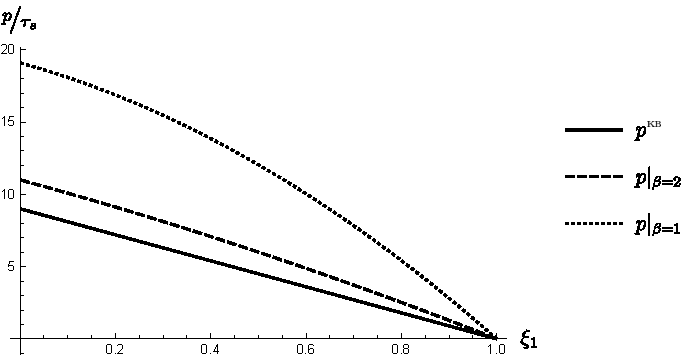
\includegraphics[scale=1.3]{./ch1/pressure}
  }
  \caption{Эпюры давления для случая круглого слоя}
  \label{fig:ch1/pressure}
\end{figure}

Используя то, что $\alpha(t) = \left(V \left(t_*-t\right)\right)^{3/2} \sqrt{2\pi / \mathcal{V}_0}$, где $\mathcal{V}_0$ -- объем слоя, можно установить зависимость между временем и стадией прессования:
\begin{equation}
  t_* - t \sim \frac{\text{Eu}^{\nicefrac{-2}{3\beta}}}{V}\sqrt[3]{\frac{\mathcal{V}_0}{2\pi}}
\end{equation}
